\label{sec:nonlinear}
\vspace{0.38cm}
\newline
With geometrical non-linearity, alterations regarding geometrically linear observation:
\begin{itemize}
    \item Consideration of non-linear terms of the strain tensor E (kinematics)
     \item Establishing the forces equilibrium or application of the impulse theorem in the deformed
configuration (kinetics)

\end{itemize}
We use: 

\begin{itemize}
    \item  (Total) Lagrange point of view which is also described as the material point of view
     \item Stress and strain quantities in the undeformed configuration (second Piola Kirchhoff
stress tensor and Green Lagrange strain tensor)

\end{itemize}



\subsection{Kinematics}
\begin{figure}[h]
    \centering
    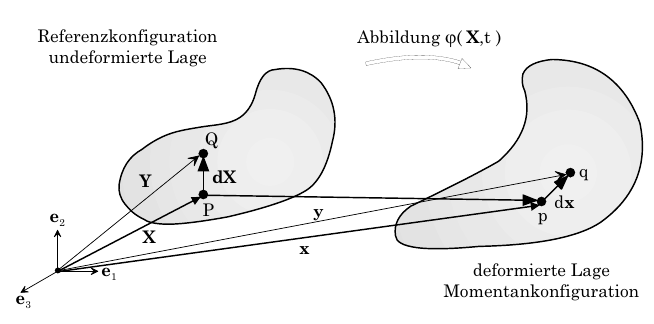
\includegraphics[scale=0.5]{Figures/Chapter2/anh3.png}
    \decoRule   
    \caption{ Current and reference configuration of a deformable material body}
    \label{fig:chap2anh3}
\end{figure}

\noindent
The fundamental of the geometrically non-linear formulation of structural mechanics is based on
the material deformation gradient F , which was already used within the scope of deriving the linear strain tensor  with the help of a non-linear deformation analysis of a material body, and
within the scope of subsequent linearization but not elaborated
because in linear observations it possesses no further significance. Non-linear observations are
a different story where the material deformation gradient defines the transformation from
reference to current configuration or from undeformed to deformed state and vice versa. These
transformations are referred to in technical literature as push forward and pull back. The
material deformation gradient is defined by a transformation of a line element dX of the
reference configuration to the current configuration dx (see figure \ref{fig:chap2anh3} ).

\begin{equation}
    dx = F \cdot dX; \quad F = \frac{{\partial x}}{{\partial X}} = \nabla x
\end{equation}
The Green Lagrange strain tensor E was also already derived and is given in equation (1.12) as function of the displacement gradient $\nabla u$ and its transpose ${\nabla ^T}u$. If we describe the
motion of the material point from the reference to the current configuration with help of the
displacement vector $\bf x = X + u$, the Green Lagrange strain tensor
\begin{equation}
    \label{5.7}
    E = \frac{1}{2}\left[ {{F^T} \cdot F - {\bf{1}}} \right] = {\nabla ^{{\rm{sym}}}}u + \frac{1}{2}{\nabla ^T}u \cdot \nabla u = \frac{1}{2}\left[ {{\nabla ^T}u + \nabla u + {\nabla ^T}u \cdot \nabla u} \right]
\end{equation}
can be represented as a function of the material deformation gradient.
\begin{equation}
 \boldsymbol{F}=\frac{\partial}{\partial \boldsymbol{X}}(\boldsymbol{X}+\boldsymbol{u})=\mathbf{1}+\nabla \boldsymbol{u} 
\end{equation}
According to this relation, the components of the term
\begin{equation}
 \nabla^{\operatorname{sym}} \boldsymbol{u}=\left[\begin{array}{ccc}u_{1,1} & \frac{1}{2}\left(u_{1,2}+u_{2,1}\right) & \frac{1}{2}\left(u_{1,3}+u_{3,1}\right) \\ \frac{1}{2}\left(u_{1,2}+u_{2,1}\right) & u_{2,2} & \frac{1}{2}\left(u_{2,3}+u_{3,2}\right) \\ \frac{1}{2}\left(u_{1,3}+u_{3,1}\right) & \frac{1}{2}\left(u_{2,3}+u_{3,2}\right) & u_{3,3}\end{array}\right] 
\end{equation}
of the linear part of the strain tensor E, given explicitly in equations (1.13) and (1.14), are
supplemented by the term $1/2 \nabla^T u$ · $\nabla u$, in the scope of geometrically non-linear theory, which can again be calculated with the displacement vector gradient according to eq. (1.7)
\begin{equation}
 \nabla \boldsymbol{u}=\left[\begin{array}{lll}u_{1,1} & u_{1,2} & u_{1,3} \\ u_{2,1} & u_{2,2} & u_{2,3} \\ u_{3,1} & u_{3,2} & u_{3,3}\end{array}\right] 
\end{equation}
by matrix multiplication.
\begin{equation}
 \frac{1}{2} \nabla^{T} \boldsymbol{u} \cdot \nabla \boldsymbol{u}=\frac{1}{2}\left[\begin{array}{lll}u_{k, 1}u_{k, 1} & u_{k, 1}u_{k, 2} & u_{k, 1} u_{k, 3} \\ u_{k, 2}u_{k, 1} & u_{k, 2}u_{k, 2} & u_{k, 2}u_{k, 3} \\ u_{k, 3}u_{k, 1} & u_{k, 3}u_{k, 2} & u_{k, 3}u_{k, 3}\end{array}\right] 
\end{equation}
It should be noted that the summation is performed over $k = 1, 2, 3$, respectively. The component presentation of the Green Lagrange strain tensor finally yields the following:
\begin{equation}
\label{5.12}
 E_{i j}=\frac{1}{2}\left(u_{i, j}+u_{j, i}+u_{k, i} u_{k, j}\right); \qquad \boldsymbol{E}=E_{i j} \boldsymbol{E}_{i} \otimes \boldsymbol{E}_{j} 
\end{equation}
In order to formulate the non-linear Finite Element methods, it remains to convert the calculation rule of the strain tensor, given in eq. (\ref{5.7}) or (\ref{5.12}), into the calculation rule of the strain
vector in a suitable way . The linear part of the strain tensor can be expressed as a vector by
application of the differential operator $D_\varepsilon$ to the displacement vector u, as described in eq.
(1.16). However, for the non-linear part of the strain tensor, no suitable operator presentation
can be found.
\begin{equation}
\label{5.13}
    {\bf{E}}({\bf{u}}) = \left[ {\begin{array}{*{20}{c}}
{{E_{11}}}\\
{{E_{22}}}\\
{{E_{33}}}\\
{2{E_{12}}}\\
{2{E_{23}}}\\
{2{E_{13}}}
\end{array}} \right] = \left[ {\begin{array}{*{20}{c}}
{{u_{1,1}}}\\
{{u_{2,2}}}\\
{{u_{3,3}}}\\
{{u_{1,2}} + {u_{2,1}}}\\
{{u_{2,3}} + {u_{3,2}}}\\
{{u_{1,3}} + {u_{3,1}}}
\end{array}} \right] + \left[ {\begin{array}{*{20}{l}}
{1/2\left( {{u_{1,1}}{u_{1,1}} + {u_{2,1}}{u_{2,1}} + {u_{3,1}}{u_{3,1}}} \right)}\\
{1/2\left( {{u_{1,2}}{u_{1,2}} + {u_{2,2}}{u_{2,2}} + {u_{3,2}}{u_{3,2}}} \right)}\\
{1/2\left( {{u_{1,3}}{u_{1,3}} + {u_{2,3}}{u_{2,3}} + {u_{3,3}}{u_{3,3}}} \right)}\\
{{u_{1,1}}{u_{1,2}} + {u_{2,1}}{u_{2,2}} + {u_{3,1}}{u_{3,2}}}\\
{{u_{1,2}}{u_{1,3}} + {u_{2,2}}{u_{2,3}} + {u_{3,2}}{u_{3,3}}}\\
{{u_{1,1}}{u_{1,3}} + {u_{2,1}}{u_{2,3}} + {u_{3,1}}{u_{3,3}}}
\end{array}} \right]{\rm{ }}
\end{equation}
According to eq (\ref{5.13}), the Green Lagrange strain tensor of geometrically non-linear
deformations is obtained by addition of the well-known linear part ${\bf D}_\varepsilon \bf u$ and the non-linear part $\bf E^\textnormal{nl}(u)$,
\begin{equation}
 \boldsymbol{E}(\boldsymbol{u})=\mathbf{D}_{\varepsilon} \boldsymbol{u}+\boldsymbol{E}^{n l}(\boldsymbol{u}) 
\end{equation}
where  ${\bf D}_\varepsilon \bf u$ and $\bf E^\textnormal{nl}(u)$ are defined as follows (summation over $k = 1, 2, 3$).

\begin{equation}
    {{\bf{D}}_\varepsilon }{\bf{u}} = \left[ {\begin{array}{*{20}{c}}
{{u_{1,1}}}\\
{{u_{2,2}}}\\
{{u_{3,3}}}\\
{{u_{1,2}} + {u_{2,1}}}\\
{{u_{2,3}} + {u_{3,2}}}\\
{{u_{1,3}} + {u_{3,1}}}
\end{array}} \right]\qquad {{\bf{E}}^{nl}}({\bf{u}}) = \left[ {\begin{array}{*{20}{l}}
{1/2}{{u_{k,1}}}{{u_{k,1}}}\\
{1/2}{{u_{k,2}}}{{u_{k,2}}}\\
{1/2}{{u_{k,3}}}{{u_{k,3}}}\\
{{u_{k,1}}}{{u_{k,2}}}{}\\
{{u_{k,2}}}{{u_{k,3}}}{}\\
{{u_{k,1}}}{{u_{k,3}}}{}
\end{array}} \right]
\end{equation}
